\chapter{Multi-Functional Optimization}
\label{chap:multi-functional_optimization}
With the single-functional optimization methods working, they can now be combined into a multi-functional optimization. To achieve this, the two separate functions need to be combined into a single function where an optimum can be determined. The weight method has been discussed in chapter \ref{chap:methods_for_optimization} and has been utilized for this thesis. 

Another method that could be used is the constraint method, where one function acts as a constraint on the other. However, the problem with this method is that the resulting optimal structure will satisfy one constraint, but not the other. The trade-off between the two may be too strict on the unconstrained function. Figure \ref{fig:constraint_optimal_point} shows that the constraint method can find points on the Pareto front, but they do not have a minimum error from an unobtainable utopia point. It is still possible to iterate towards the true minimum, but the weight was chosen for its elegance. 
\begin{figure}[ht]
    \centering
    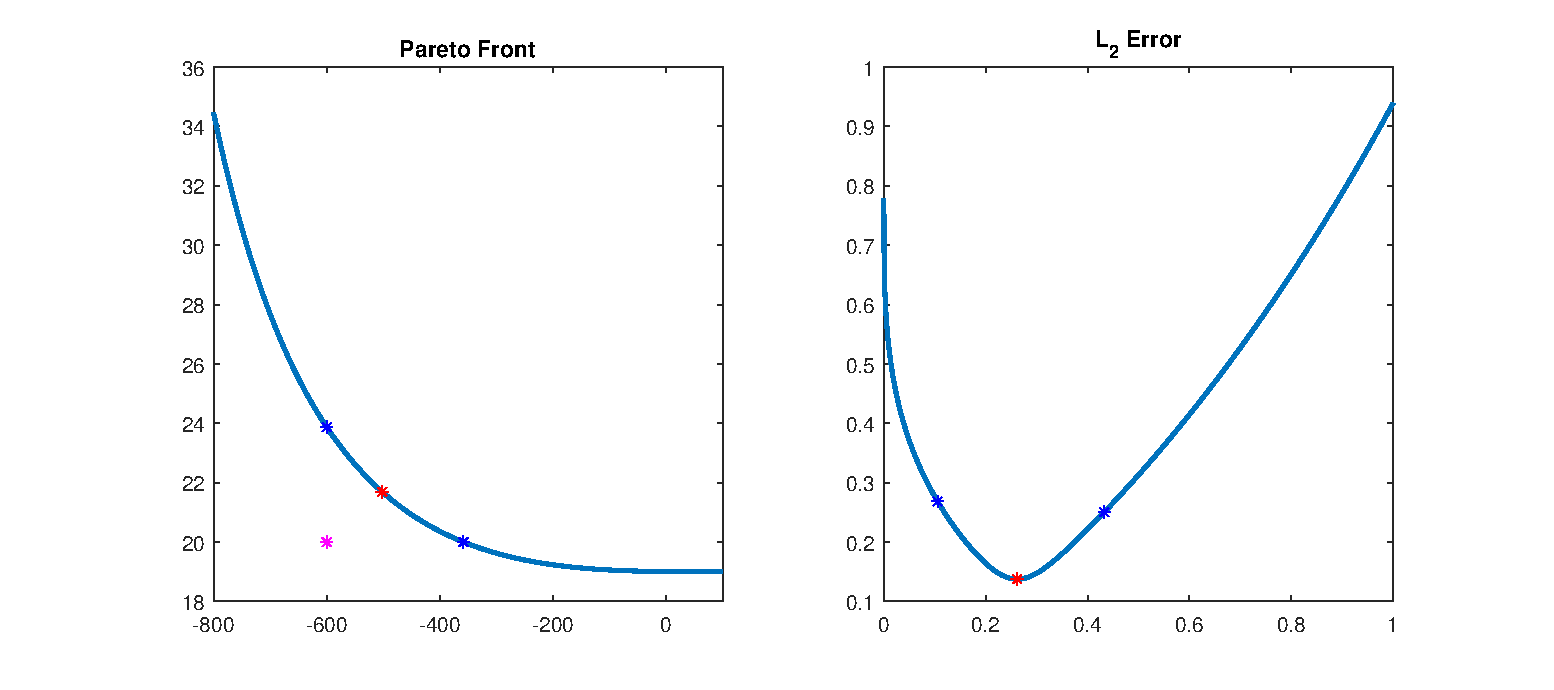
\includegraphics[width=0.95\linewidth]{figures/chapter_5/ConstraintMethoLimitation.eps}
    \caption{Pareto front showing points obtained from constraint method (blue) and the real optimum (red) given an unobtainable utopia point (magenta).}
    \label{fig:constraint_optimal_point}
\end{figure}


\section{Pareto Front Generation}
As was mentioned, in this thesis, the weight method is used for generating Pareto optimal points. The sum of the weights should add to one \cite{Kochenderfer_Wheeler_2019}. The weight method converts the multiple objective functions into a single equation that can then be optimized using techniques already discussed in chapter \ref{chap:methods_for_optimization}. Equation \ref{eq:single_function_objective} shows the single objective function applied to the normalized thermal ($c^*_t$) and structural ($c^*_s$) compliance.
\begin{equation}
    J(w,\rho) = w c^*_t(\rho) + (1 - w)c^*_s(\rho)
    \label{eq:single_function_objective}
\end{equation}

To obtain reasonable results, the functions are normalized so that the compliance of each is of a similar order. This also ensures the gradients of each separate objective function are of a similar order. For the sensitivity analysis, equation \ref{eq:single_function_objective} is differentiated w.r.t the relative density, $\rho$, as shown in equation \ref{eq:single_function_objective_gradient}.
\begin{equation}
    \frac{\partial J}{\partial\rho} = w\frac{\partial c^*_t}{\partial\rho} + (1-w)\frac{\partial c^*_s}{\partial\rho}
    \label{eq:single_function_objective_gradient}
\end{equation}

With that, a Pareto front can be generated by varying the weight between 0 and 1, where the extremes would return to the single-function objective. Figure \ref{fig:mf_pareto_front_simple_domain} shows the Pareto front generated for setup shown in \ref{fig:simple_domain}. In this simulation, conductivity and stiffness were maximized for a given weight.
\begin{figure}[ht]
    \centering
    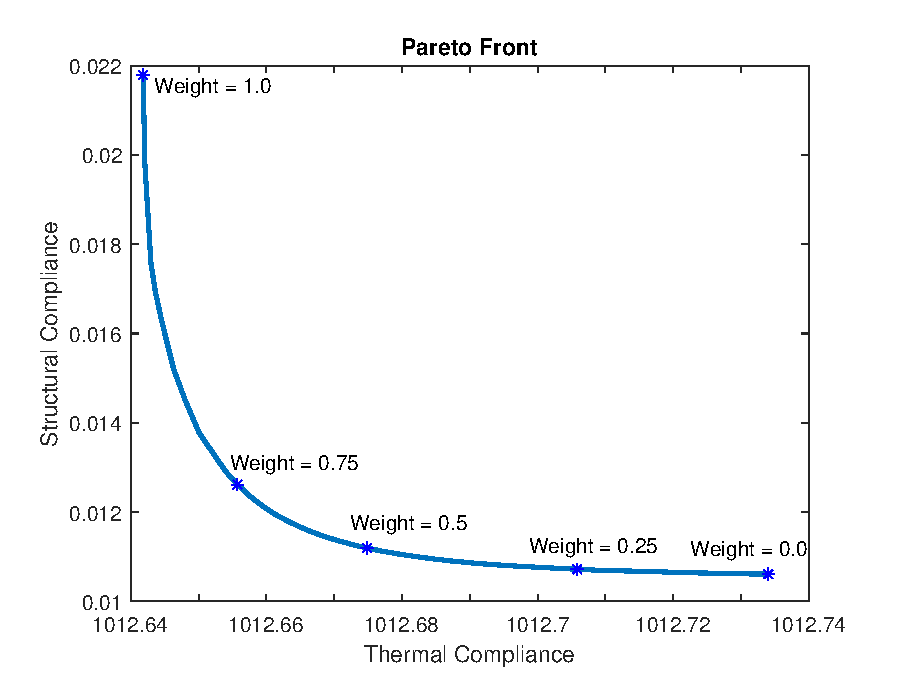
\includegraphics[width=0.6\linewidth]{figures/chapter_5/ParetoFrontForGivenStructures.eps}
    \caption{Pareto Front for Given Domain}
    \label{fig:mf_pareto_front_simple_domain}
\end{figure}

Figure \ref{fig:multi-functional_optimum_progression} shows the gradual transition from a thermal optimum to a structural optimum. The porosity range for these structures was set to 5\% to 20\%. With this range, as has already been discussed, the structures can have \emph{'disconnected'} regions, and a lack of branches and struts. These results are valid, as has already been shown in chapter \ref{chap:singe_functional_optimization}.
\begin{figure}[ht]
    \centering
    \begin{subfigure}[b]{0.45\linewidth}
        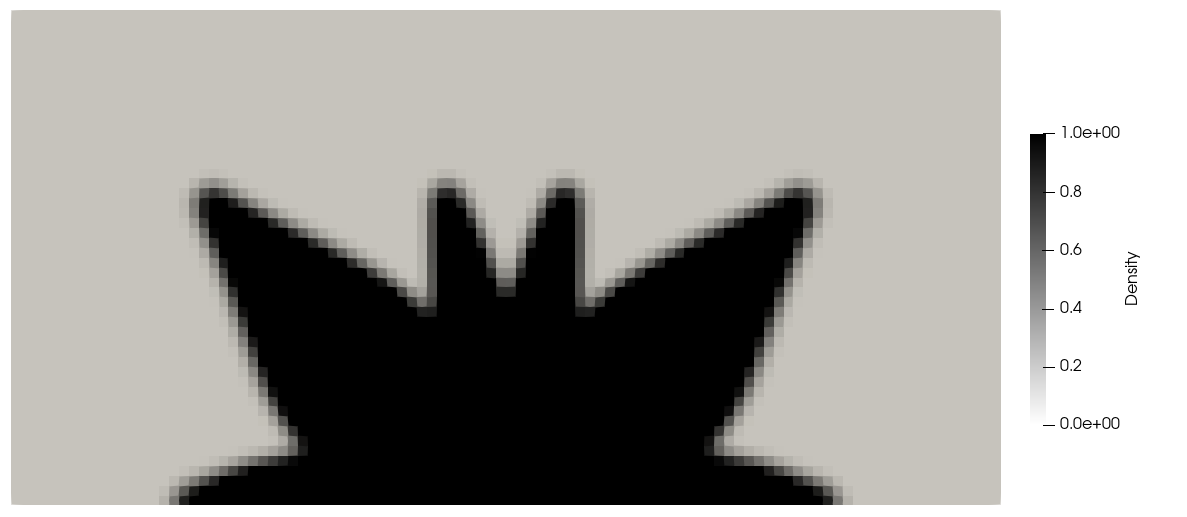
\includegraphics[width=\linewidth]{figures/chapter_5/MF_1to0.png}
        \caption{Weight of 1}
    \end{subfigure}
    \hfill
    \begin{subfigure}[b]{0.45\linewidth}
        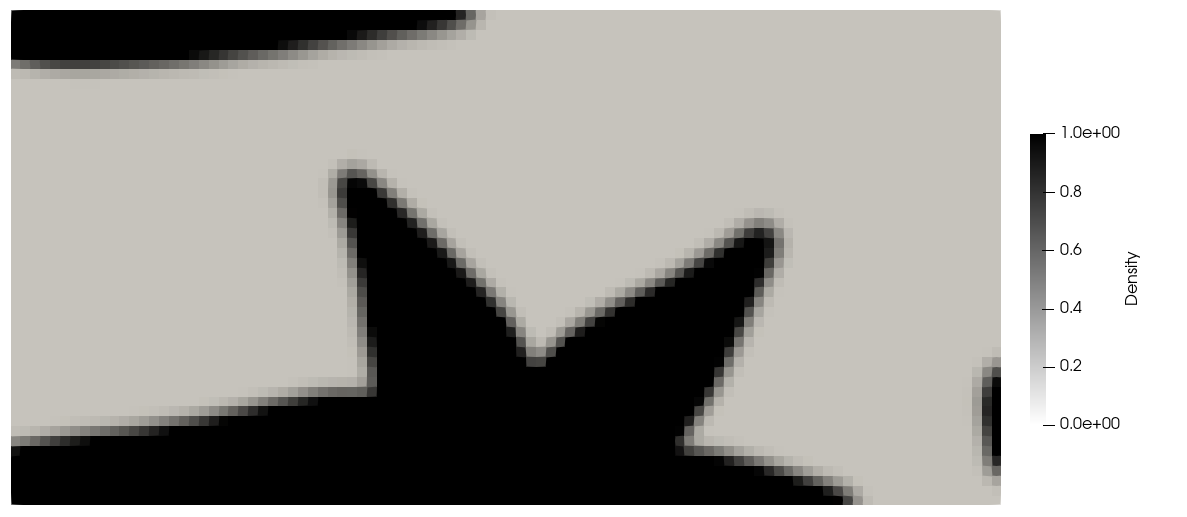
\includegraphics[width=\linewidth]{figures/chapter_5/MF_3to1.png}
        \caption{Weight of 0.75}
    \end{subfigure}

    \centering
    \begin{subfigure}[b]{0.45\linewidth}
        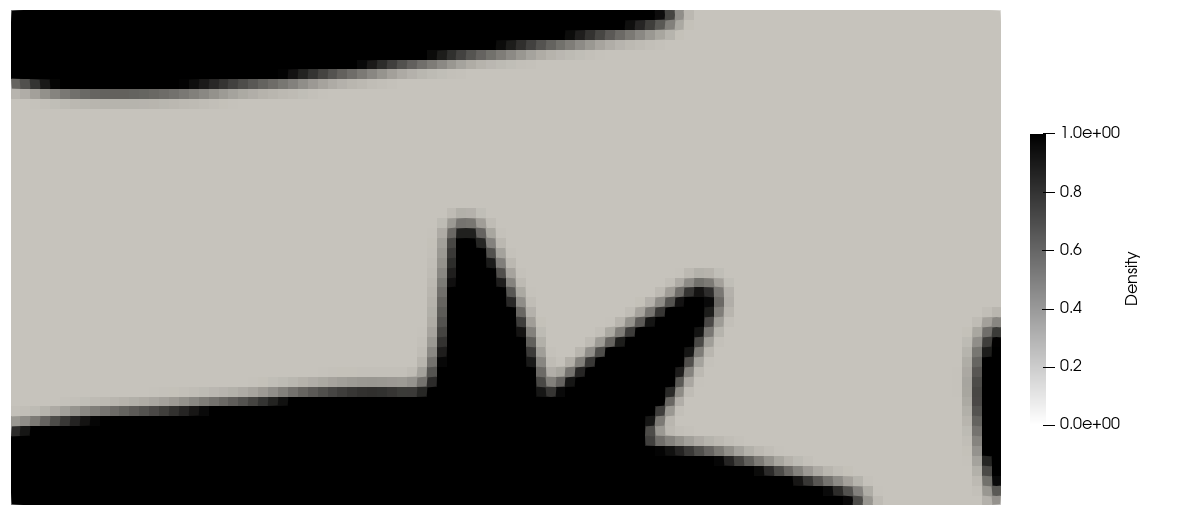
\includegraphics[width=\linewidth]{figures/chapter_5/MF_1to1.png}
        \caption{Weight of 0.5}
    \end{subfigure}
    \hfill
    \begin{subfigure}[b]{0.45\linewidth}
        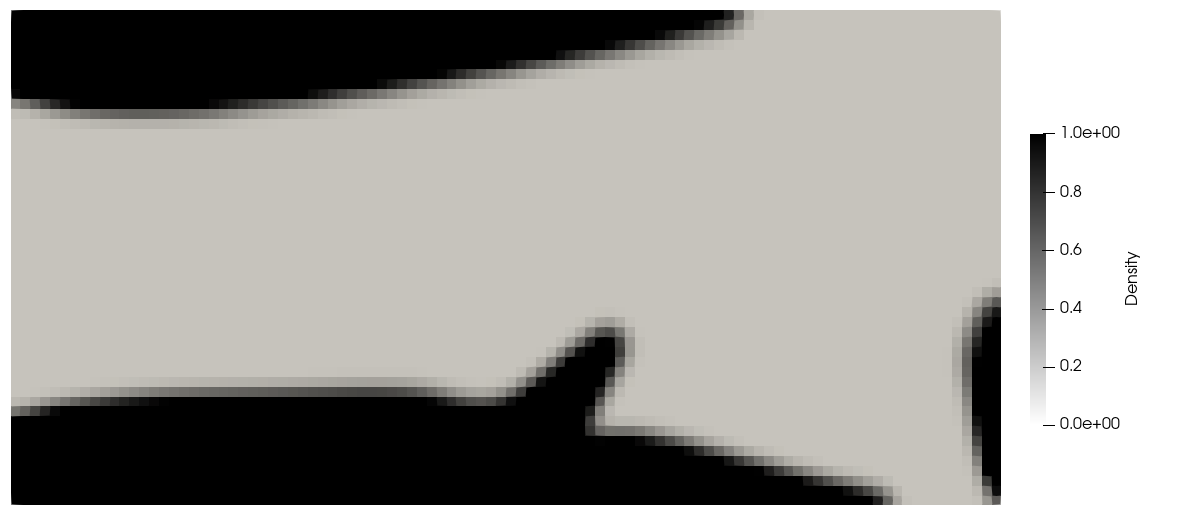
\includegraphics[width=\linewidth]{figures/chapter_5/MF_1to3.png}
        \caption{Weight of 0.25}
    \end{subfigure}

    \centering
    \begin{subfigure}[b]{0.45\linewidth}
        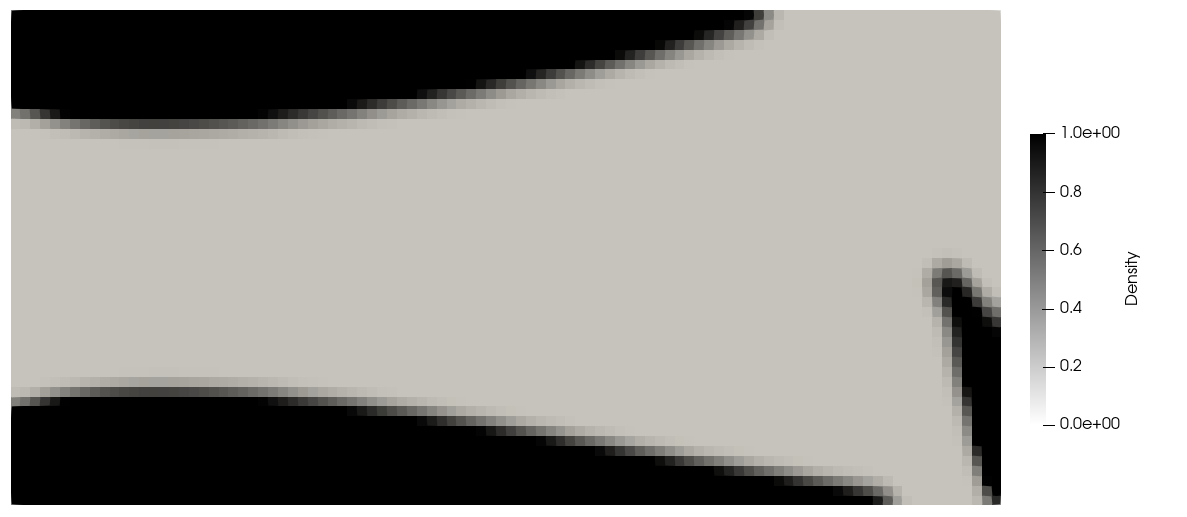
\includegraphics[width=\linewidth]{figures/chapter_5/MF_0to1.png}
        \caption{Weight of 0}
    \end{subfigure}
    \caption{The gradual progression from thermal to structural optimum obtained from the Pareto front generation}
    \label{fig:multi-functional_optimum_progression}
\end{figure}


\section{Determining Optimum Trade-off}
While the Pareto-front can be generated for a given number of weights, it is a time-consuming process that is not guaranteed to find a true optimum. Instead, a combination of methods can be used to get as close to a minimum as possible. It is important to realize that the compliance of each problem is not known without first performing a topology optimization. The shape of the Pareto front is also not known without constructing it as discussed previously. Instead, a strategy to iteratively find an optimum has been proposed in this thesis.

Assuming the Pareto-front is convex, there will be one point of minimal error. Therefore, the rate of convergence will depend on how accurate the initial guess is. To even begin to have an idea of an initial guess, the bounds of the Pareto front should be known. It is unlikely they can be determined from experience because depending on the forces, heat flux, and shape of the domain, the bounds of the Pareto front could be anything. Instead, the bounds are first determined by optimizing the single-functional problems, as has been done by Pejman and Najafi, \cite{Pejman_Najafi_2023}. This gives the range of compliance for each problem, which also allows the single-functional problems to be normalized. 

To make an educated initial guess of the optimal point, the utopia point is projected onto the line segment that can be constructed from the bounding points. Due to the shape of the Pareto front, this guess is usually quite inaccurate, but at least a rough estimate is now possible. Figure \ref{fig:optimal_point_construction} illustrates the bounding points being determined, the line segment being constructed, and the projected utopia point.
\begin{figure}[ht]
    \centering
    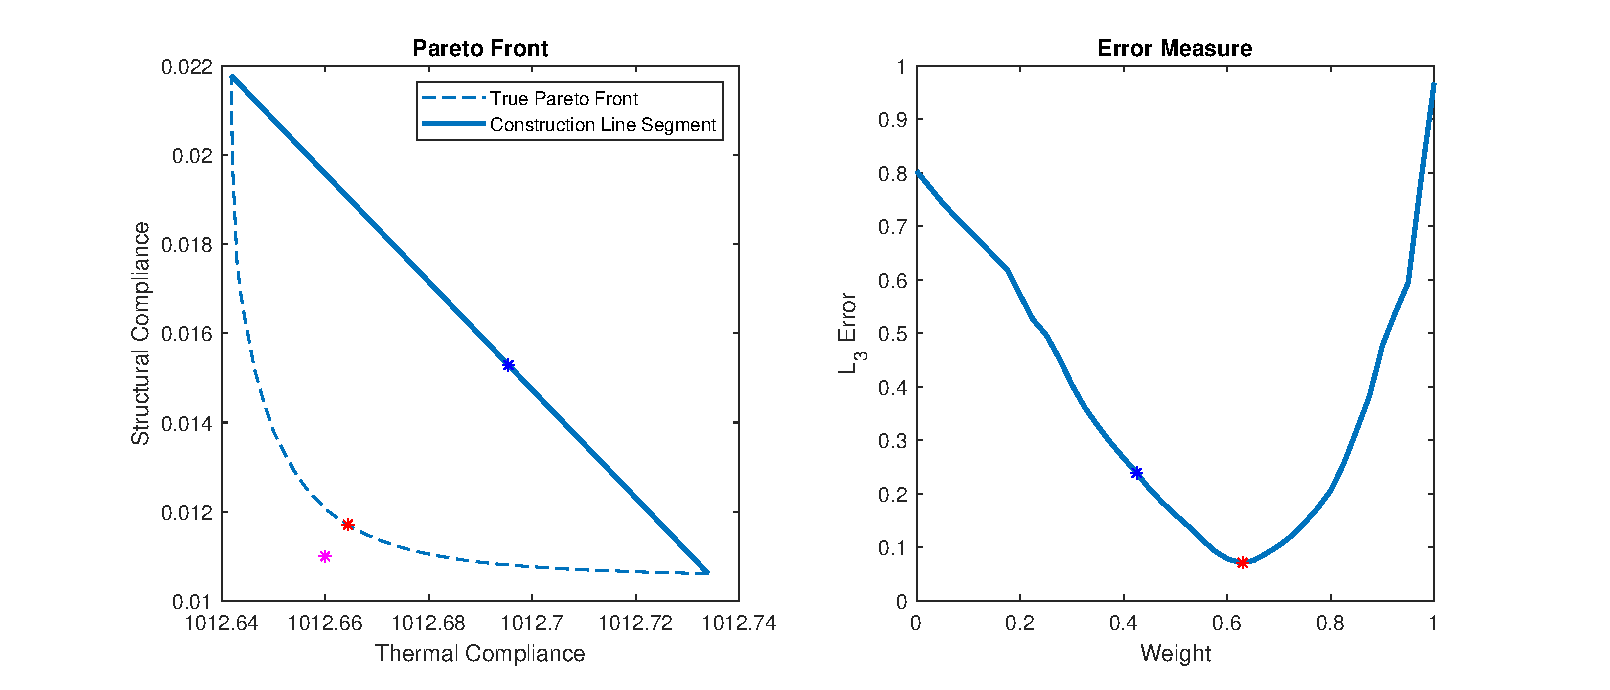
\includegraphics[width=0.85\linewidth]{figures/chapter_5/OptimalPointConstruction.eps}
    \caption{Initial guess (blue point) based on projecting the utopia point (magenta) onto the construction line (solid blue)}
    \label{fig:optimal_point_construction}
\end{figure}

To iterate towards the true optimum, the quadratic fit method, described by Kochenderfer, et al., \cite{Kochenderfer_Wheeler_2019} has been utilized. This method is a gradient-free bracketing method that uses information from three points to construct a parabola and then finds its minimum.
\begin{figure}[ht]
    \centering
    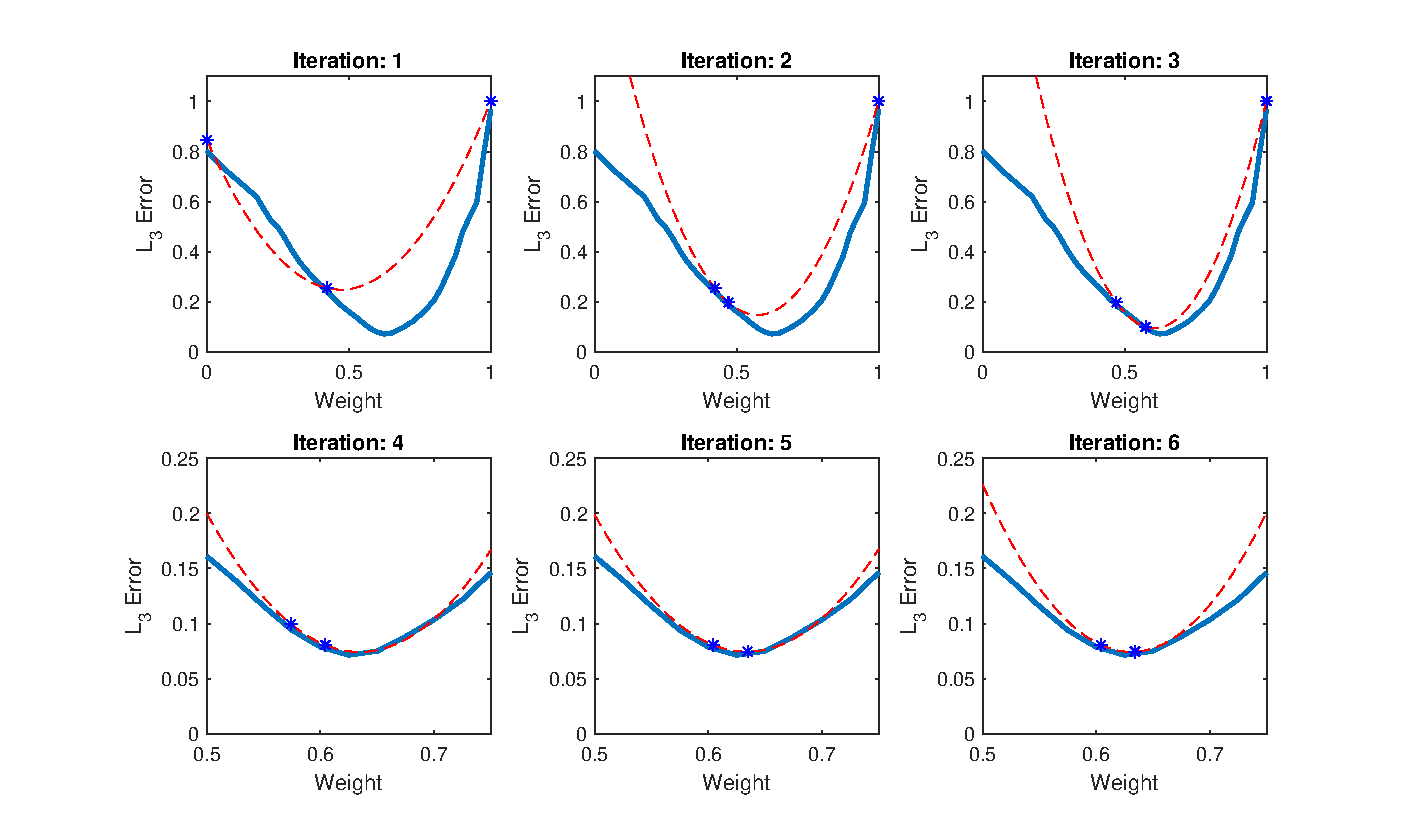
\includegraphics[width=0.85\linewidth]{figures/chapter_5/QuadraticFitConvergence.eps}
    \caption{Quadratic fit convergence showing the real error norm (solid blue) and the fitted parabolas (dashed red) constructed by three points (red star)}
    \label{fig:quadratic_fit_method}
\end{figure}

It turns out that generally the error measure very roughly resembles a parabola, so this method can find the true optimal point, given a reasonable tolerance, in very few iterations. This method works by updating the bounds of the parabola each iteration, and will eventually collapse around the optimal point. Figure \ref{fig:quadratic_fit_method} shows how this method converges toward the optimal point. The convergence plot shows that it is already near the optimal point after three iterations, and after five iterations the optimal point is already determined within a low tolerance. 

\subsection*{Limitations}
This method does have some drawbacks. When the optimal point is, or is near the bounding points, a couple of problems can arise. Figure \ref{fig:optimal_point_is_bounding_point} illustrates when this problem can arise. The first problem is that the projection method that is used means the initial guess may be outside the allowable weight range. To solve this issue, the initial guess can be limited to a range such as $w_\text{guess} \in [0.1, 0.9]$. The quadratic fit method can then continue as normal.

The second issue with having the optimal point near the bounding points is that the quadratic fit method might find a minimum that is outside the allowable weight range. To overcome this issue, a bisection is performed instead to update the central point in the parabola. This can be repeated until the method converges to the true optimum, or until the quadratic fit method finds a valid optimal point. Note that the weight range can not be limited for this case, because the optimum could be the bounding point.

\begin{figure}[ht]
    \centering
    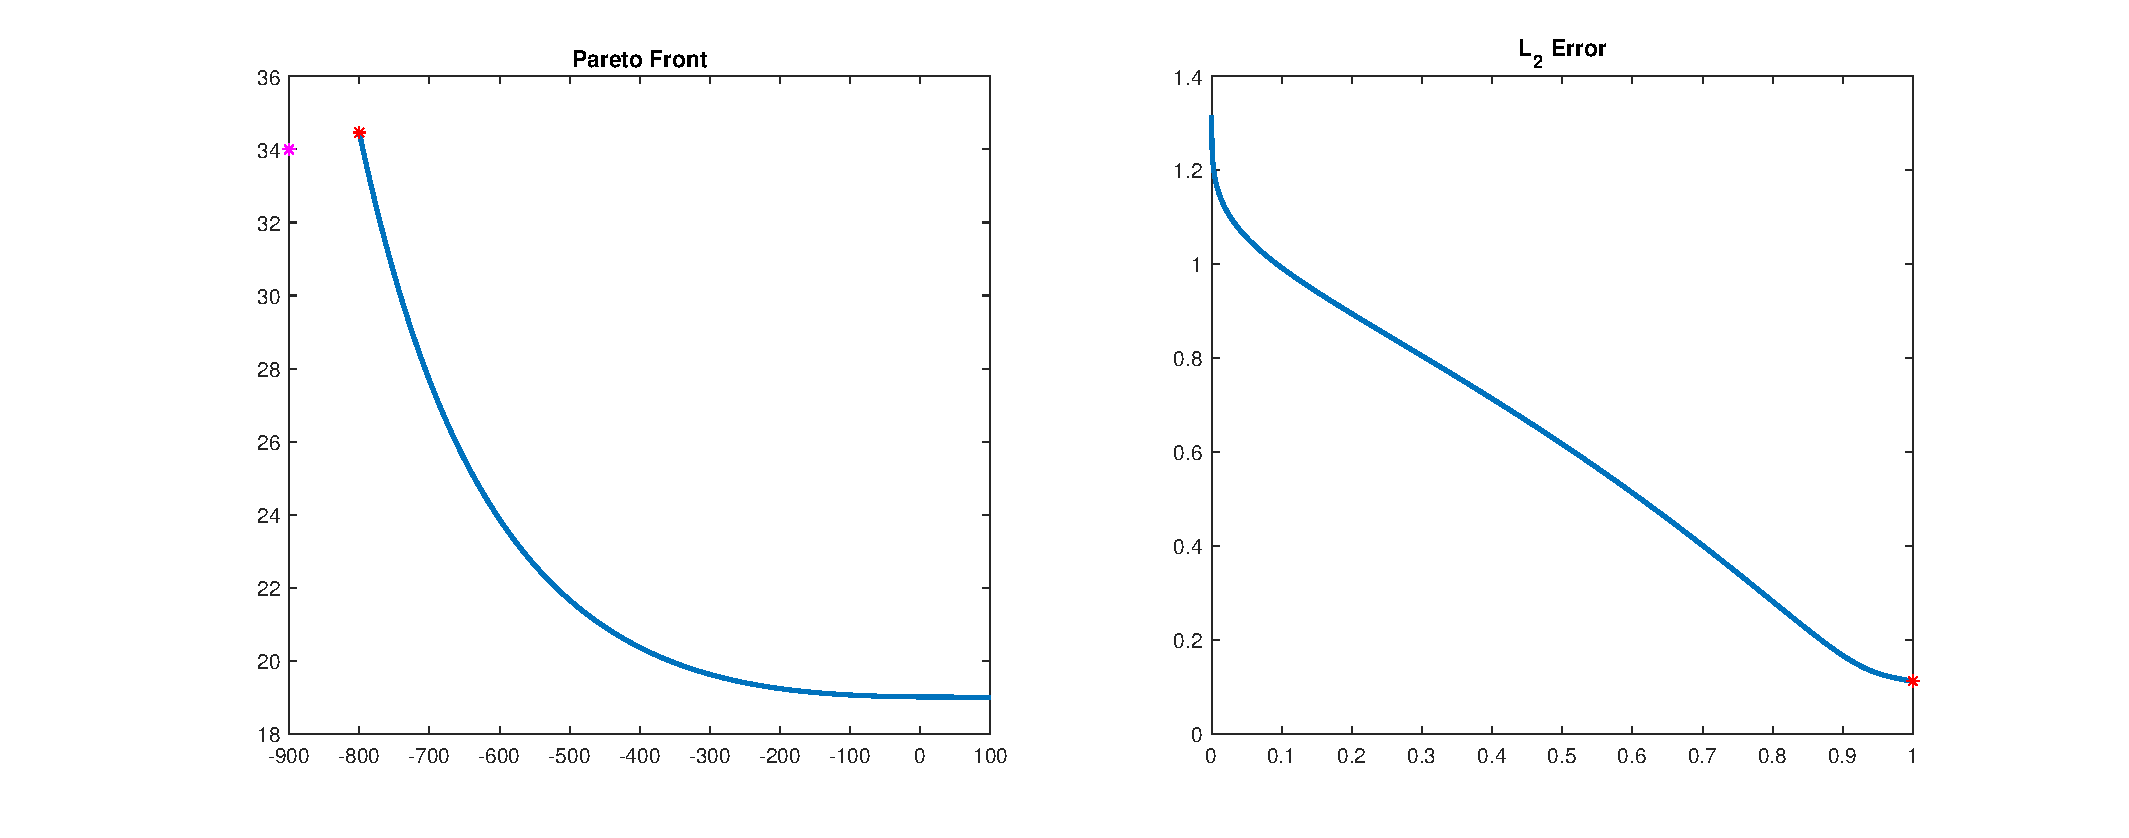
\includegraphics[width=0.9\linewidth]{figures/chapter_5/BoundingPointOptimum.eps}
    \caption{Limitation where the bounding point is the optimal point}
    \label{fig:optimal_point_is_bounding_point}
\end{figure}

Another limitation is that many local minima could be present when the function is concave. In such a situation, a more accurate initial guess is required to ensure it converges to the correct minimum. Through some experimentation, however, the Pareto front is usually convex. This is because the two functions tend to contribute to each other, rather than compete.


\section{Maximizing Thermal Conductivity and Stiffness}
The algorithms developed in chapter \ref{chap:singe_functional_optimization} were for the minimization of thermal and structural compliance, as well as the minimization of phase-change compliance. This section discusses results obtained using the minimization of thermal and structural compliance.

\subsection*{Test Case 1}
To illustrate the effectiveness of the selected method, two test cases have been produced for the same Pareto front. The first utopia point was set to $U(1012.66, 0.011)$. The bounds of the Pareto front a then determined, and the compliances are normalised. The optimal point is then iteratively determined. This case converges to a reasonable tolerance in three iterations.
\begin{figure}[ht]
    \centering
    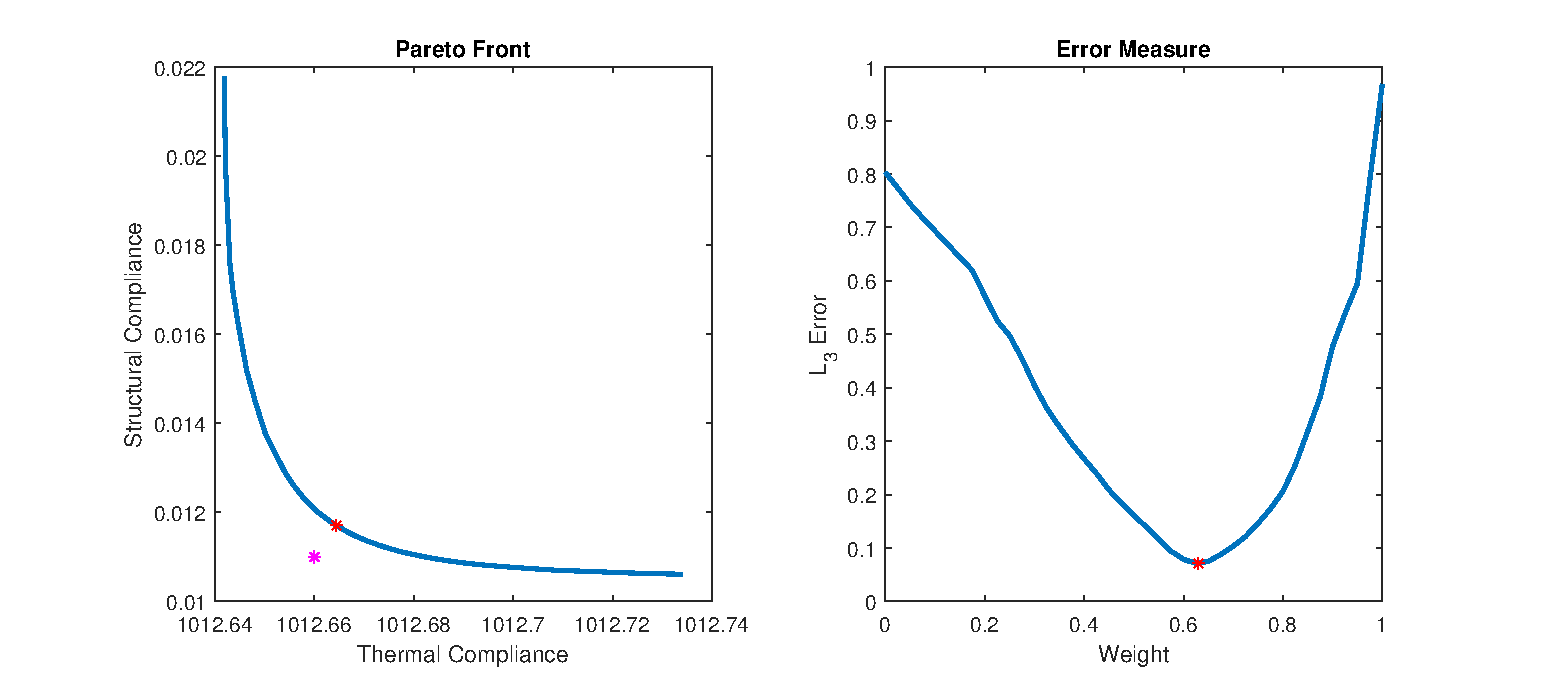
\includegraphics[width=0.8\linewidth]{figures/chapter_5/ParetoOpt_w0063.eps}
    \caption{Optimum obtained (red) for utopia point $U(1012.66, 0.011)$ (magenta)}
    \label{fig:utopia_66_011}
\end{figure}

Figure \ref{fig:optimal_structure_1} shows the structure that was generated. Compared to figure \ref{fig:multi-functional_optimum_progression}, this structure lies somewhere between structures b and c as is expected. 
\begin{figure}[ht]
    \centering
    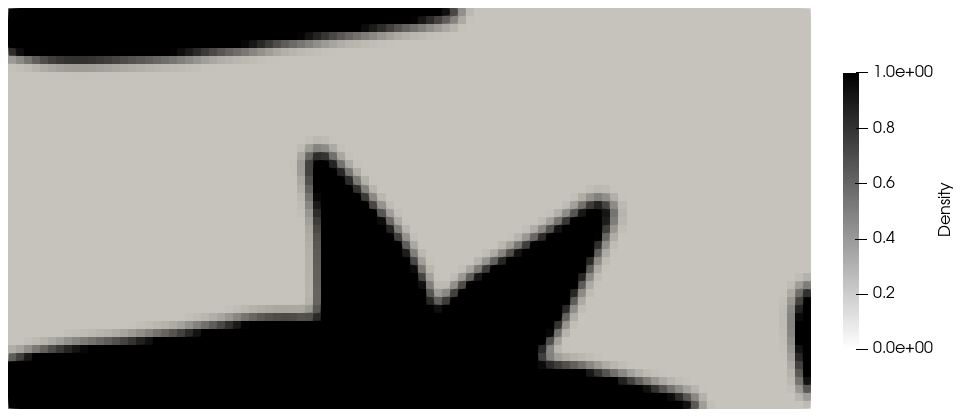
\includegraphics[width=0.7\linewidth]{figures/chapter_5/ParetoOptimuim_Test1.png}
    \caption{Pareto-optimal structure obtained for utopia point $U(1012.66, 0.011)$}
    \label{fig:optimal_structure_1}
\end{figure}


\subsection*{Test Case 2}
In this test case, the utopia point was set to $U(1012.64, 0.014)$. This case has a much sharper error norm but still converges to the optimal point in very few iterations. The optimal point is determined with a coarse tolerance in only six iterations, and to a high resolution in nine.
\begin{figure}[ht]
    \centering
    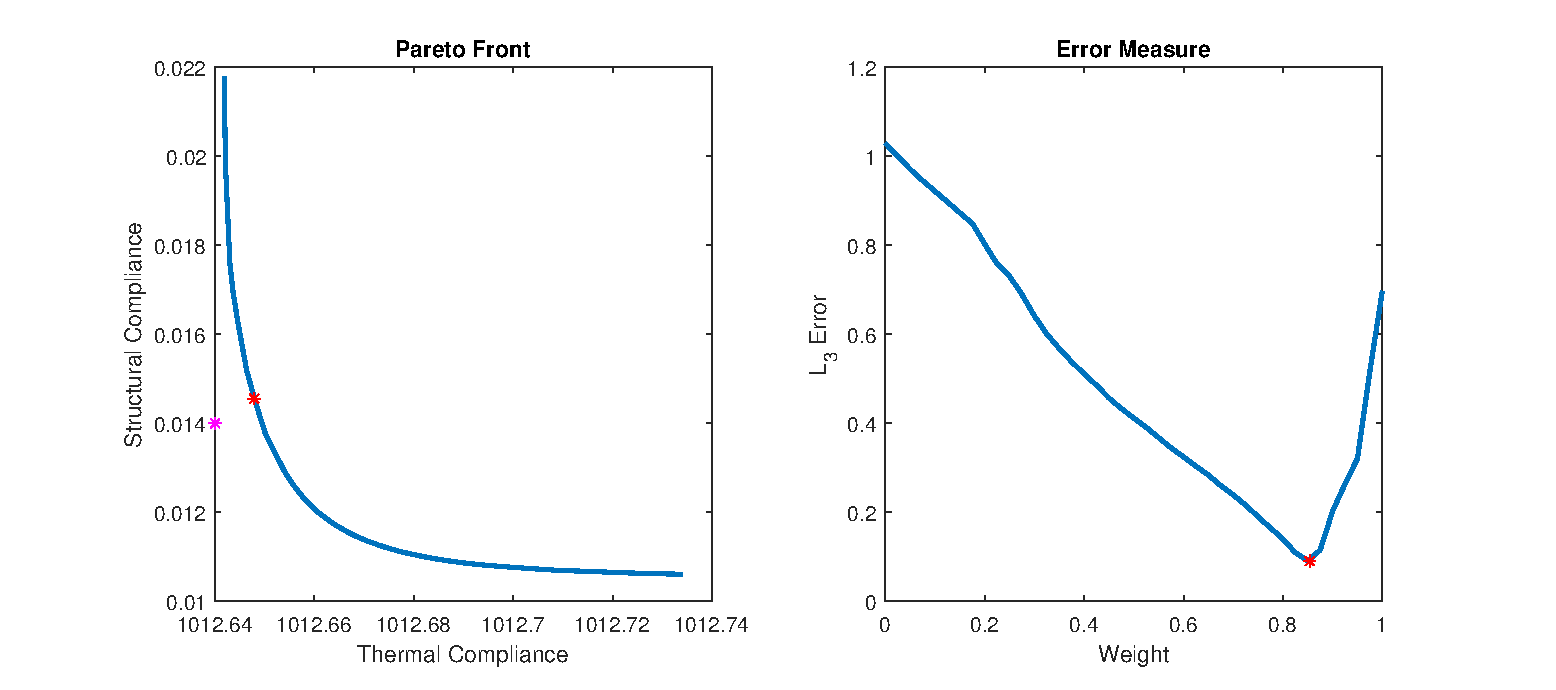
\includegraphics[width=0.8\linewidth]{figures/chapter_5/ParetoOpt_w00854.eps}
    \caption{Optimum obtained (red) for utopia point $U(1012.64, 0.014)$ (magenta)}
    \label{fig:utopia_64_014}
\end{figure}

Figure \ref{fig:optimal_structure_2} shows the structure generated. This structure lies between structures a and b which is expected. 
\begin{figure}[ht]
    \centering
    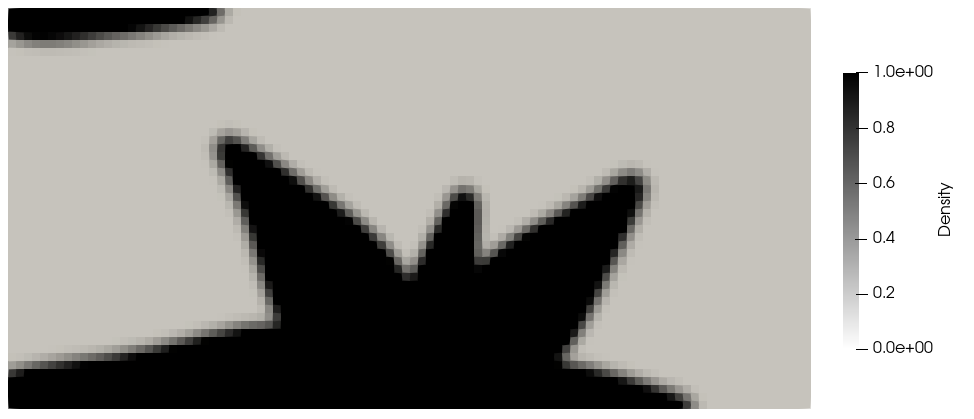
\includegraphics[width=0.7\linewidth]{figures/chapter_5/ParetoOptimuim_Test2.png}
    \caption{Pareto-optimal structure obtained for utopia point $U(1012.64,0.014)$}
    \label{fig:optimal_structure_2}
\end{figure}

The two test cases that have been used for the simple domain show that an optimum can be found. Both optimal structures were found in only a few iterations. However, to ensure generability, more test cases have been produced with different boundary conditions in chapter \ref{chap:test_cases}.


\section{Minimising Temperature and Maximising Stiffness}
This section discusses results obtained where the phase-change compliance and structural compliance were objective functions. This section expands on observations made in chapter \ref{chap:singe_functional_optimization} where the phase change compliance optimization provided some benefits. Unfortunately, to generate a Pareto front in a reasonable amount of time, the coarsest mesh had to be used. This makes it difficult to compare results with the previous section, but the overall structure is still visible.

Figure \ref{fig:multi-functional_pc_progression} shows some of the intermediate structures that have been generated using the Pareto front generation tool. These structures were optimized until the time the domain fully melted, as this provided the most benefit as shown in figure \ref{fig:phase_change_optimal_comparison}. The progression from thermal to structural optimum is clear. Because of the chosen end time, the thermal optimum has two branches that fill much of the domain.
\begin{figure}[ht]
    \centering
    \begin{subfigure}[b]{0.45\linewidth}
        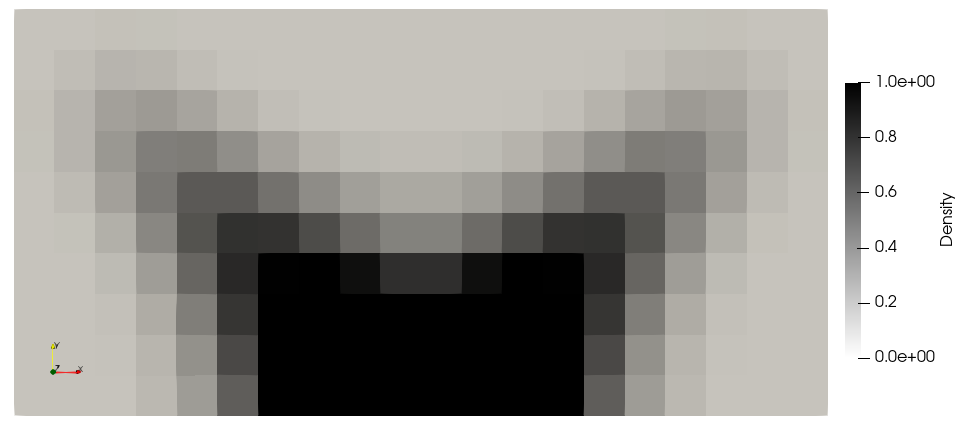
\includegraphics[width=\linewidth]{figures/chapter_5/PC_MF_1to0.png}
        \caption{Weight of 1}
    \end{subfigure}
    \hfill
    \begin{subfigure}[b]{0.45\linewidth}
        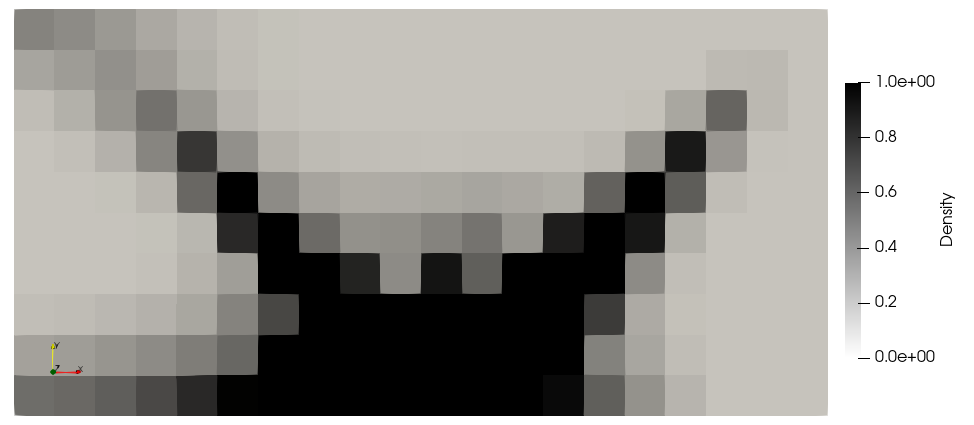
\includegraphics[width=\linewidth]{figures/chapter_5/PC_MF_3to1.png}
        \caption{Weight of 0.75}
    \end{subfigure}
    
    \begin{subfigure}[b]{0.45\linewidth}
        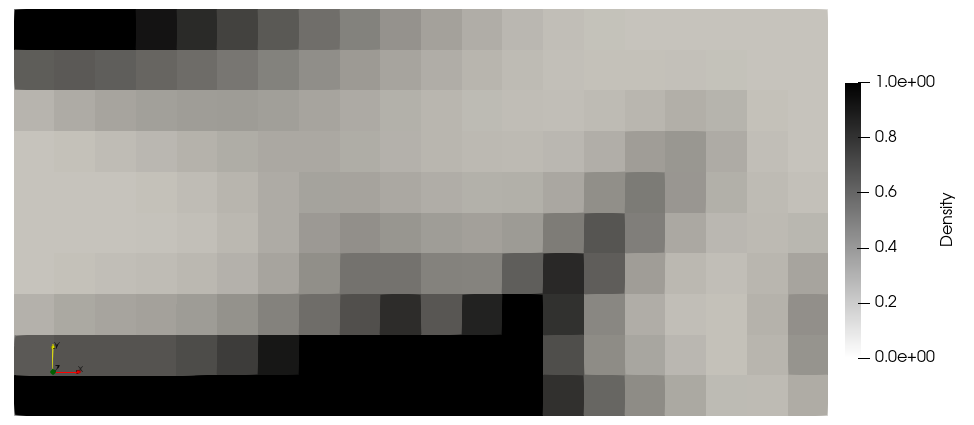
\includegraphics[width=\linewidth]{figures/chapter_5/PC_MF_1to1.png}
        \caption{Weight of 0.5}
    \end{subfigure}
    \hfill
    \begin{subfigure}[b]{0.45\linewidth}
        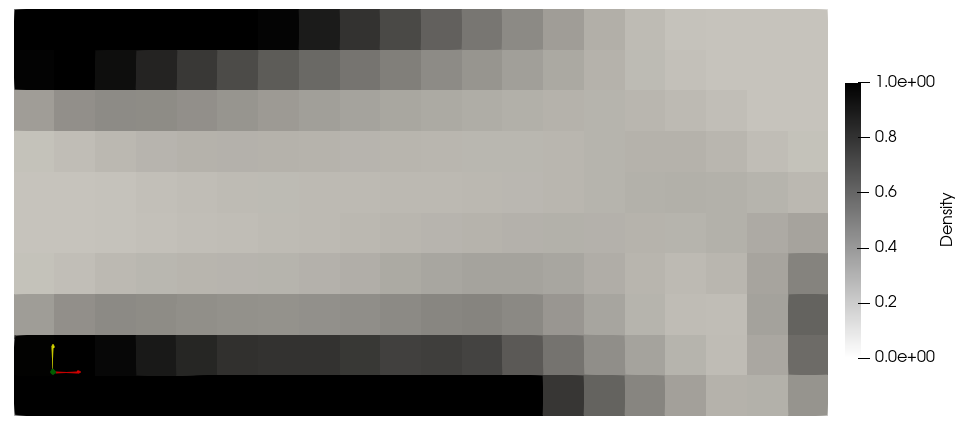
\includegraphics[width=\linewidth]{figures/chapter_5/PC_MF_1to3.png}
        \caption{Weight of 0.25}
    \end{subfigure}
    
    \begin{subfigure}[b]{0.45\linewidth}
        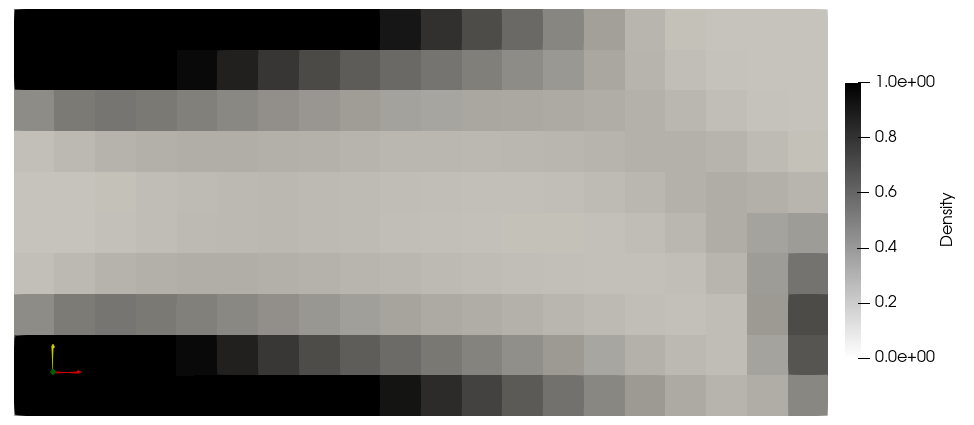
\includegraphics[width=\linewidth]{figures/chapter_5/PC_MF_0to1.png}
        \caption{Weight of 0}
    \end{subfigure}
    \caption{The gradual progression from phase-change to structural optimum from the Pareto front generation}
    \label{fig:multi-functional_pc_progression}
\end{figure}

To compare the results to the conductivity optimal structures, a new set of structures was generated for the former case, and the phase change results have been plotted in figure \ref{fig:phase_change_results_coarsest}. This plot shows different weight ratios. The plot shows that the weight has a much less linear relationship with the phase-change optimizer than with the conductivity optimizer. These results shown in the plot are therefore not directly relatable, but they do show that the limits in optimums are comparable.
\begin{figure}[ht]
    \centering
    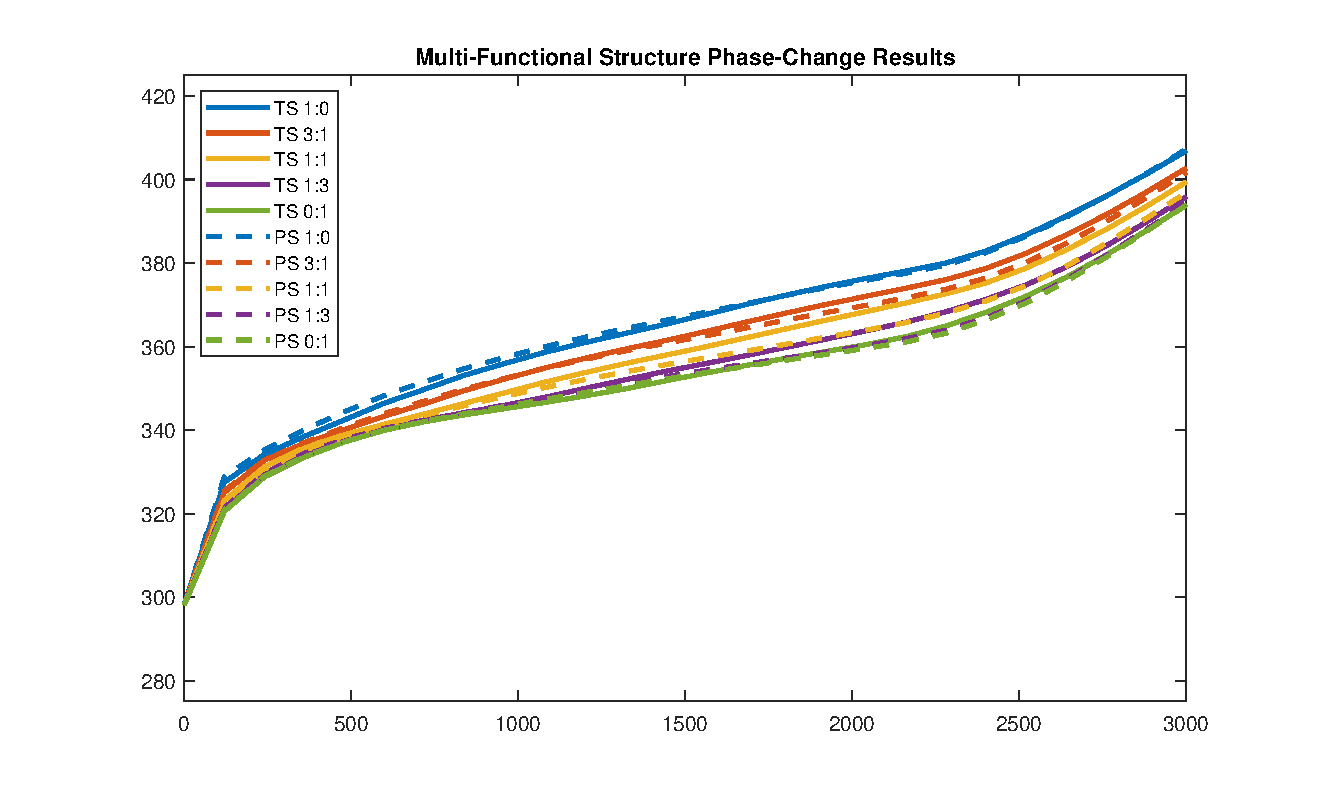
\includegraphics[width=0.7\linewidth]{figures/chapter_5/PhaseChangeResultsCoarsest.eps}
    \caption{Phase change results showing the maximum temperature in the domain for the maximization of thermal conductivity and stiffness (TS/solid lines), and optimization of phase change compliance and stiffness (PS/dashed lines)}
    \label{fig:phase_change_results_coarsest}
\end{figure}

\subsection*{Test Case}
Finally, a Pareto optimal structure has been generated for the utopia point $U(212500, 0.012)$. As has been discussed, first the bounds of the Pareto front are determined, the compliances are normalized, and the optimal point is iteratively determined. The algorithm returned in six iterations but with relatively poor accuracy.
\begin{figure}[ht]
    \centering
    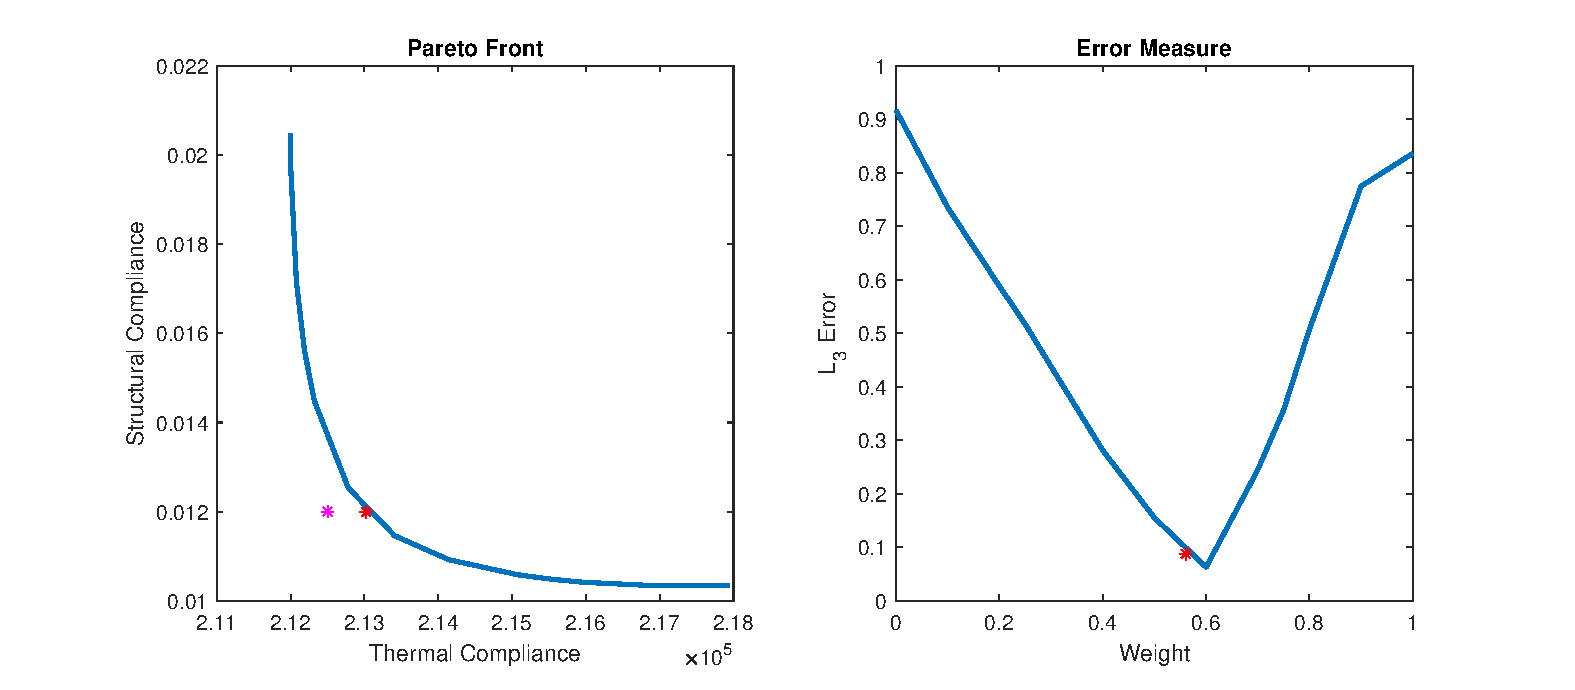
\includegraphics[width=0.8\linewidth]{figures/chapter_5/ParetoOpt_PC.eps}
    \caption{Optimum obtained (red) for utopia point $U(212500,0.012)$ (magenta)}
    \label{fig:pareto_optimum_phase_change}
\end{figure}

Figure \ref{fig:pareto_optimal_structure_pc} shows the structure that is obtained. It resembles a structure between figure \ref{fig:multi-functional_pc_progression} b and c. This is expected because the optimal weight is found to be around $w=0.56$.
\begin{figure}[ht]
    \centering
    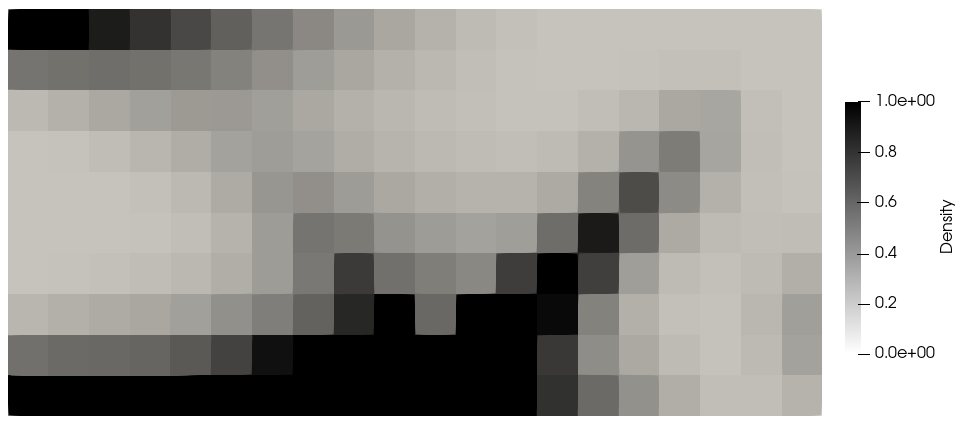
\includegraphics[width=0.6\linewidth]{figures/chapter_5/ParetoOptimum_PhaseChange.png}
    \caption{Pareto-optimal structure obtained for utopia point $U(212500,0.012)$}
    \label{fig:pareto_optimal_structure_pc}
\end{figure}


\section{Remarks}
While the phase-change-structural optimization algorithm does provide a small benefit, the computational costs make it prohibitive to use more extensively. One of the major limiting factors is that the mesh needs to be quite coarse to obtain a structure in a reasonable amount of time. As the benefit is so negligible, in the following chapter, only structures obtained for the maximization of thermal conductivity and stiffness will be generated.

As was mentioned in this thesis, de-homogenization was not a major focus of this thesis because the types of cells were already defined. To illustrate a basic de-homogenization of the structure, figure \ref{fig:dehomogenized_optimal_pc_structure}. This structure is simple to generate because the positions and radius of each unit cell are determined by the mesh. This figure also helps to illustrate that the empty regions in the relative density plot are actually populated by high-porosity unit cells.
\begin{figure}[ht]
    \centering
    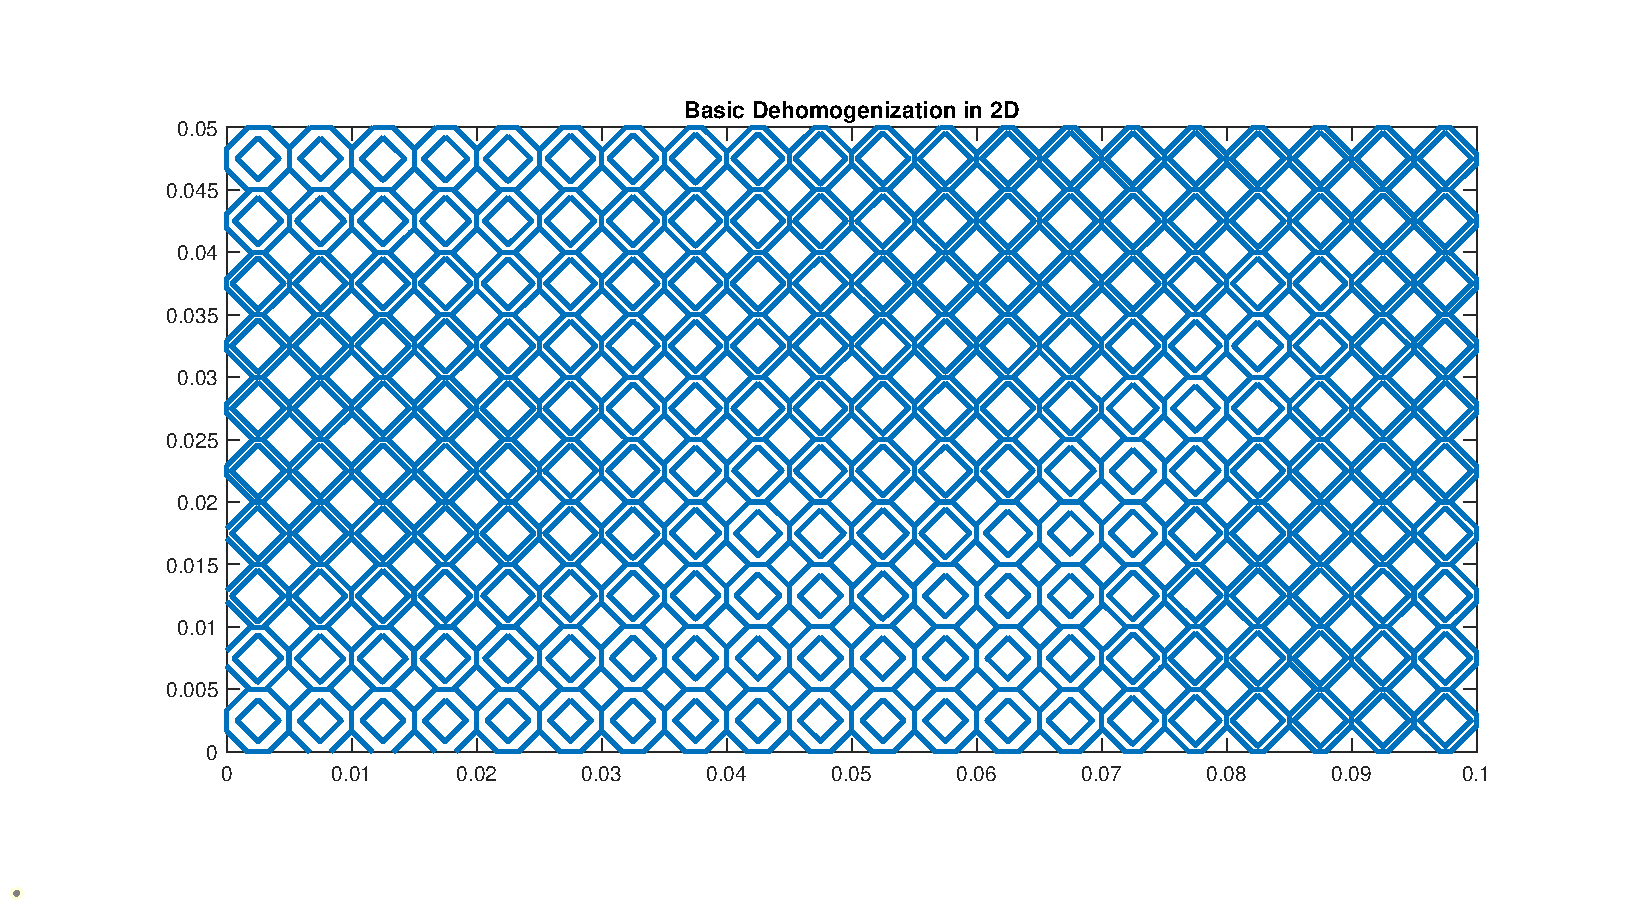
\includegraphics[width=0.7\linewidth]{figures/chapter_5/BasicDehomogenization.eps}
    \caption{Basic de-homogenization of structure shown in figure \ref{fig:pareto_optimal_structure_pc}}
    \label{fig:dehomogenized_optimal_pc_structure}
\end{figure} 